% do not remove begin
%% Verze pro jednostranný tisk:
% Okraje: levý 40mm, pravý 25mm, horní a dolní 25mm
% (ale pozor, LaTeX si sám přidává 1in)
%\documentclass[12pt,a4paper]{report}
%\setlength\textwidth{145mm}
%\setlength\textheight{247mm}
%\setlength\oddsidemargin{15mm}
%\setlength\evensidemargin{15mm}
%\setlength\topmargin{0mm}
%\setlength\headsep{0mm}
%\setlength\headheight{0mm}
% \openright zařídí, aby následující text začínal na pravé straně knihy
%\let\openright=\clearpage

%% Pokud tiskneme oboustranně:
\documentclass[12pt,a4paper,twoside,openright]{report}
\setlength\textwidth{145mm}
\setlength\textheight{247mm}
\setlength\oddsidemargin{15mm}
\setlength\evensidemargin{0mm}
\setlength\topmargin{0mm}
\setlength\headsep{0mm}
\setlength\headheight{0mm}
\let\openright=\cleardoublepage

%% Pokud používáte csLaTeX (doporučeno):
%\usepackage{czech}
%% Pokud nikoliv:
%\usepackage[czech]{babel}
% \usepackage[T1]{fontenc}

%%%% ENCODING: usually latin2, cp1250 nebo utf8 %%%
\usepackage[utf8x]{inputenc}

%%%%% OTHER PACKAGES  %%%%%
% \usepackage{doxygen} % wrong sty! 
\usepackage{pdfpages}
\usepackage{listings}
\usepackage{color}
\usepackage{graphicx}
\usepackage{amsthm}


\usepackage{draftwatermark} 
\SetWatermarkScale{4}
\SetWatermarkLightness{0.5}
\SetWatermarkText{Draft!}

\usepackage{multirow} 
\usepackage[table]{xcolor}

\usepackage{amsmath, amsthm, amssymb}
\usepackage[round]{natbib} % citace

%% Balíček hyperref, kterým jdou vyrábět klikací odkazy v PDF,
%% ale hlavně ho používáme k uložení metadat do PDF (včetně obsahu).
%\usepackage[ps2pdf,unicode]{hyperref}   % Musí být za všemi ostatními balíčky
\usepackage[unicode]{hyperref}   % Musí být za všemi ostatními balíčky
\hypersetup{pdftitle=Diploma thesis}   % TODO check if correct
% \hypersetup{pdfauthor=Ondřej Plátek}
\hypersetup{pdfauthor=Ondrej Platek}


%%% MACROS %%%% 
% Tato makra přesvědčují mírně ošklivým trikem LaTeX, aby hlavičky kapitol
% sázel příčetněji a nevynechával nad nimi spoustu místa. Směle ignorujte.
\makeatletter
\def\@makechapterhead#1{
  {\parindent \z@ \raggedright \normalfont
   \Huge\bfseries \thechapter. #1
   \par\nobreak
   \vskip 20\p@
}}
\def\@makeschapterhead#1{
  {\parindent \z@ \raggedright \normalfont
   \Huge\bfseries #1
   \par\nobreak
   \vskip 20\p@
}}
\makeatother

% Toto makro definuje kapitolu, která není očíslovaná, ale je uvedena v obsahu.
\def\chapwithtoc#1{
\chapter*{#1}
\addcontentsline{toc}{chapter}{#1}
}

%%% TODO makra
\def\todo#1{
\emph{\color{red} TODO: #1}
}

\def\todon#1{
  \todo{#1 \\}
}
% references to footnote
% usage: \footnoteremember{myfootnote}{This is my footnote} and then \footnoterecall{myfootnote} 
\newcommand{\footnoteremember}[2]{
    \footnote{#2}
    \newcounter{#1}
    \setcounter{#1}{\value{footnote}}
}
\newcommand{\footnoterecall}[1]{
    \footnotemark[\value{#1}]
}
\graphicspath{{./images/}}

% includes file with code
% usage: \code{MyCodeName}{../testapp/models.py}
\newcommand{\code}[3]{
  \hrulefill
  \subsubsection*{#1}
  \lstinputlisting[style=#2]{#3}
  \vspace{2em}
}


%%% END OF MACROS %%%
\begin{document}


\definecolor{CDecorators}{rgb}{0.9,0.5,0.5}
\definecolor{Numbers}{rgb}{0.5,0,0}
\definecolor{MatchingBrackets}{rgb}{0.25,0.5,0.5}
\definecolor{CKeywords}{rgb}{0,0,1}
\definecolor{CSelf}{rgb}{0,1,1}
\definecolor{CStrings}{rgb}{0,0.63,0}
\definecolor{CComments}{rgb}{0,0.63,1}
\definecolor{CBackground}{rgb}{0.94,0.94,0.94}

\lstdefinestyle{C}{
language=C++,
numbers=left,
numberstyle=\tiny,
xleftmargin=4pt,
framextopmargin=2em,
framexbottommargin=2em,
showspaces=false,
showtabs=false,
showstringspaces=false,
breaklines=true,
breakatwhitespace=false,
% prebreak = \raisebox{0ex}[0ex][0ex]{\ensuremath{\hookleftarrow}},
postbreak = \raisebox{0ex}[0ex][0ex]{\ensuremath{\hookrightarrow}},
frame=l,
tabsize=4,
% Basic
basicstyle=\ttfamily\scriptsize,
backgroundcolor=\color{CBackground},
% Comments
% commentstyle=\color{CComments}\slshape,
% % Strings
stringstyle=\color{CStrings},
morekeywords={int,main},
keywordstyle={\color{CKeywords}\bfseries},
}

../text/snippets/python_style.tex
% do not remove end


% TODO create biblio compatible with citations!
% TODO look at Pasky diploma thesis
% TODO Do not number Introduction and Conclusion & number every other chapter!
% TODO look at pasky citations - quote everything 
% -> find some citation generator?
% TODO create list of abbreviations (added to content) works at Pasky
% TODO create list of Figures, and table if many (not working at Pasky)
%%% Strana s automaticky generovaným obsahem práce. U matematických
%%% prací je přípustné, aby seznam tabulek a zkratek, existují-li, byl umístěn
%%% na začátku práce, místo na jejím konci.
% TODO quote images -> use Wikipedia CC (creative commons) 
% TODO how to quota Wikipedia properly
% TODO describe in appendix source structure BUT DO NOT DESCRIBE source code itself
% ?TODO? put future work to separate chapter before conclusion?
% TODO input listings http://pedrokroger.net/2011/04/printing-python-code-with-latex/

% % !TEX root = main.tex
\pagenumbering{roman}

\begin{titlepage}
\begin{center}
\ \\

\vspace{15mm}

\large
Charles University in Prague\\
Faculty of~Mathematics and Physics\\

\vspace{5mm}

{\Large\bf MASTER THESIS}

\vspace{15mm}


\includegraphics[scale=0.4]{logo.eps} %%% source http://www.mff.cuni.cz/fakulta/symboly/logo.eps

\vspace{20mm}
%\normalsize
{\Large Ondřej Plátek}\\ 

\vspace{5mm}
{\Large\bf Automatic speech recognition using Kaldi}

\vspace{20mm}
\large
\noindent
Institute of~Formal and Applied Linguistics\\
\noindent
Supervisor: Ing. Mgr. Filip Jurčíček, Ph.D.\\
\noindent
Study branch: Theoretical Computer Science\\
\end{center}
\vspace{20mm}
\begin{center}
Prague 2013
\end{center}

\end{titlepage} % zde koncí úvodní strana

%%%%%%%% 2-3 page with master thesis task
% FIXME -remove this from electronic version%%%%% 
% \todon{Insert the~task $../images/zadani[1-2].png$ for the~printed version}

\begin{figure}[htp] \centering{
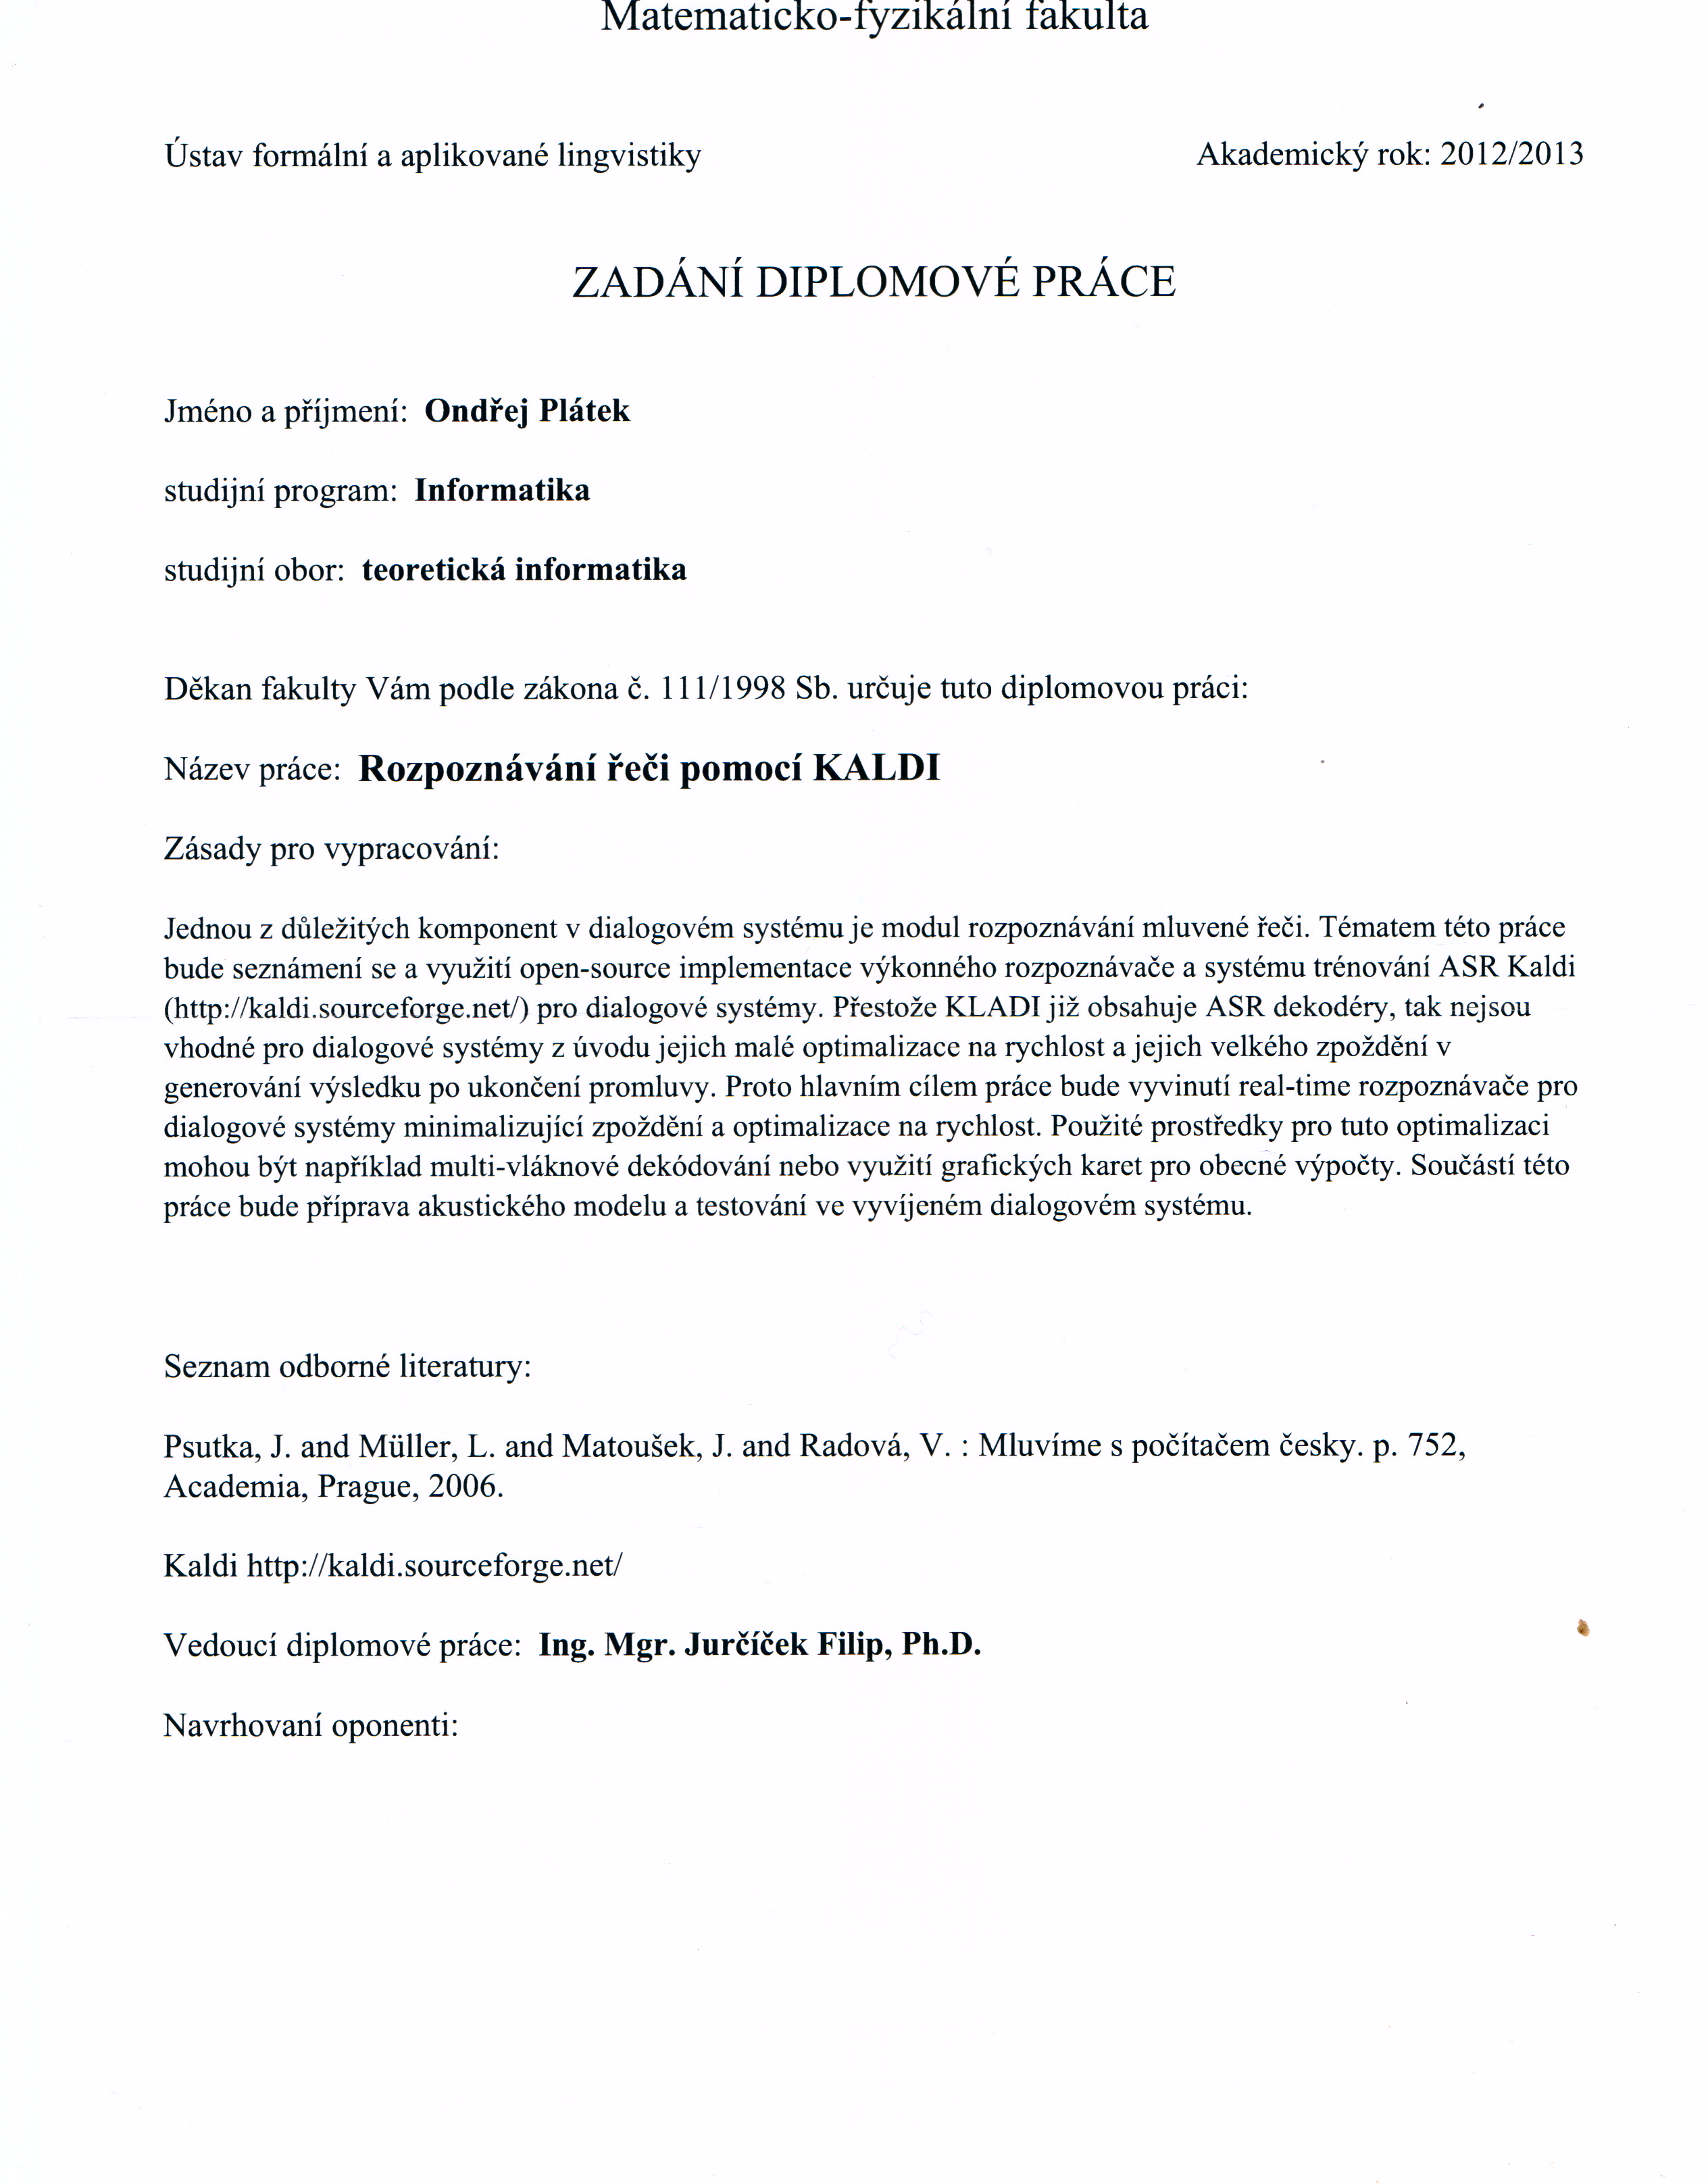
\includegraphics[scale=0.82]{zadani1}}
\end{figure}  

\newpage
\begin{figure}[htp] \centering{
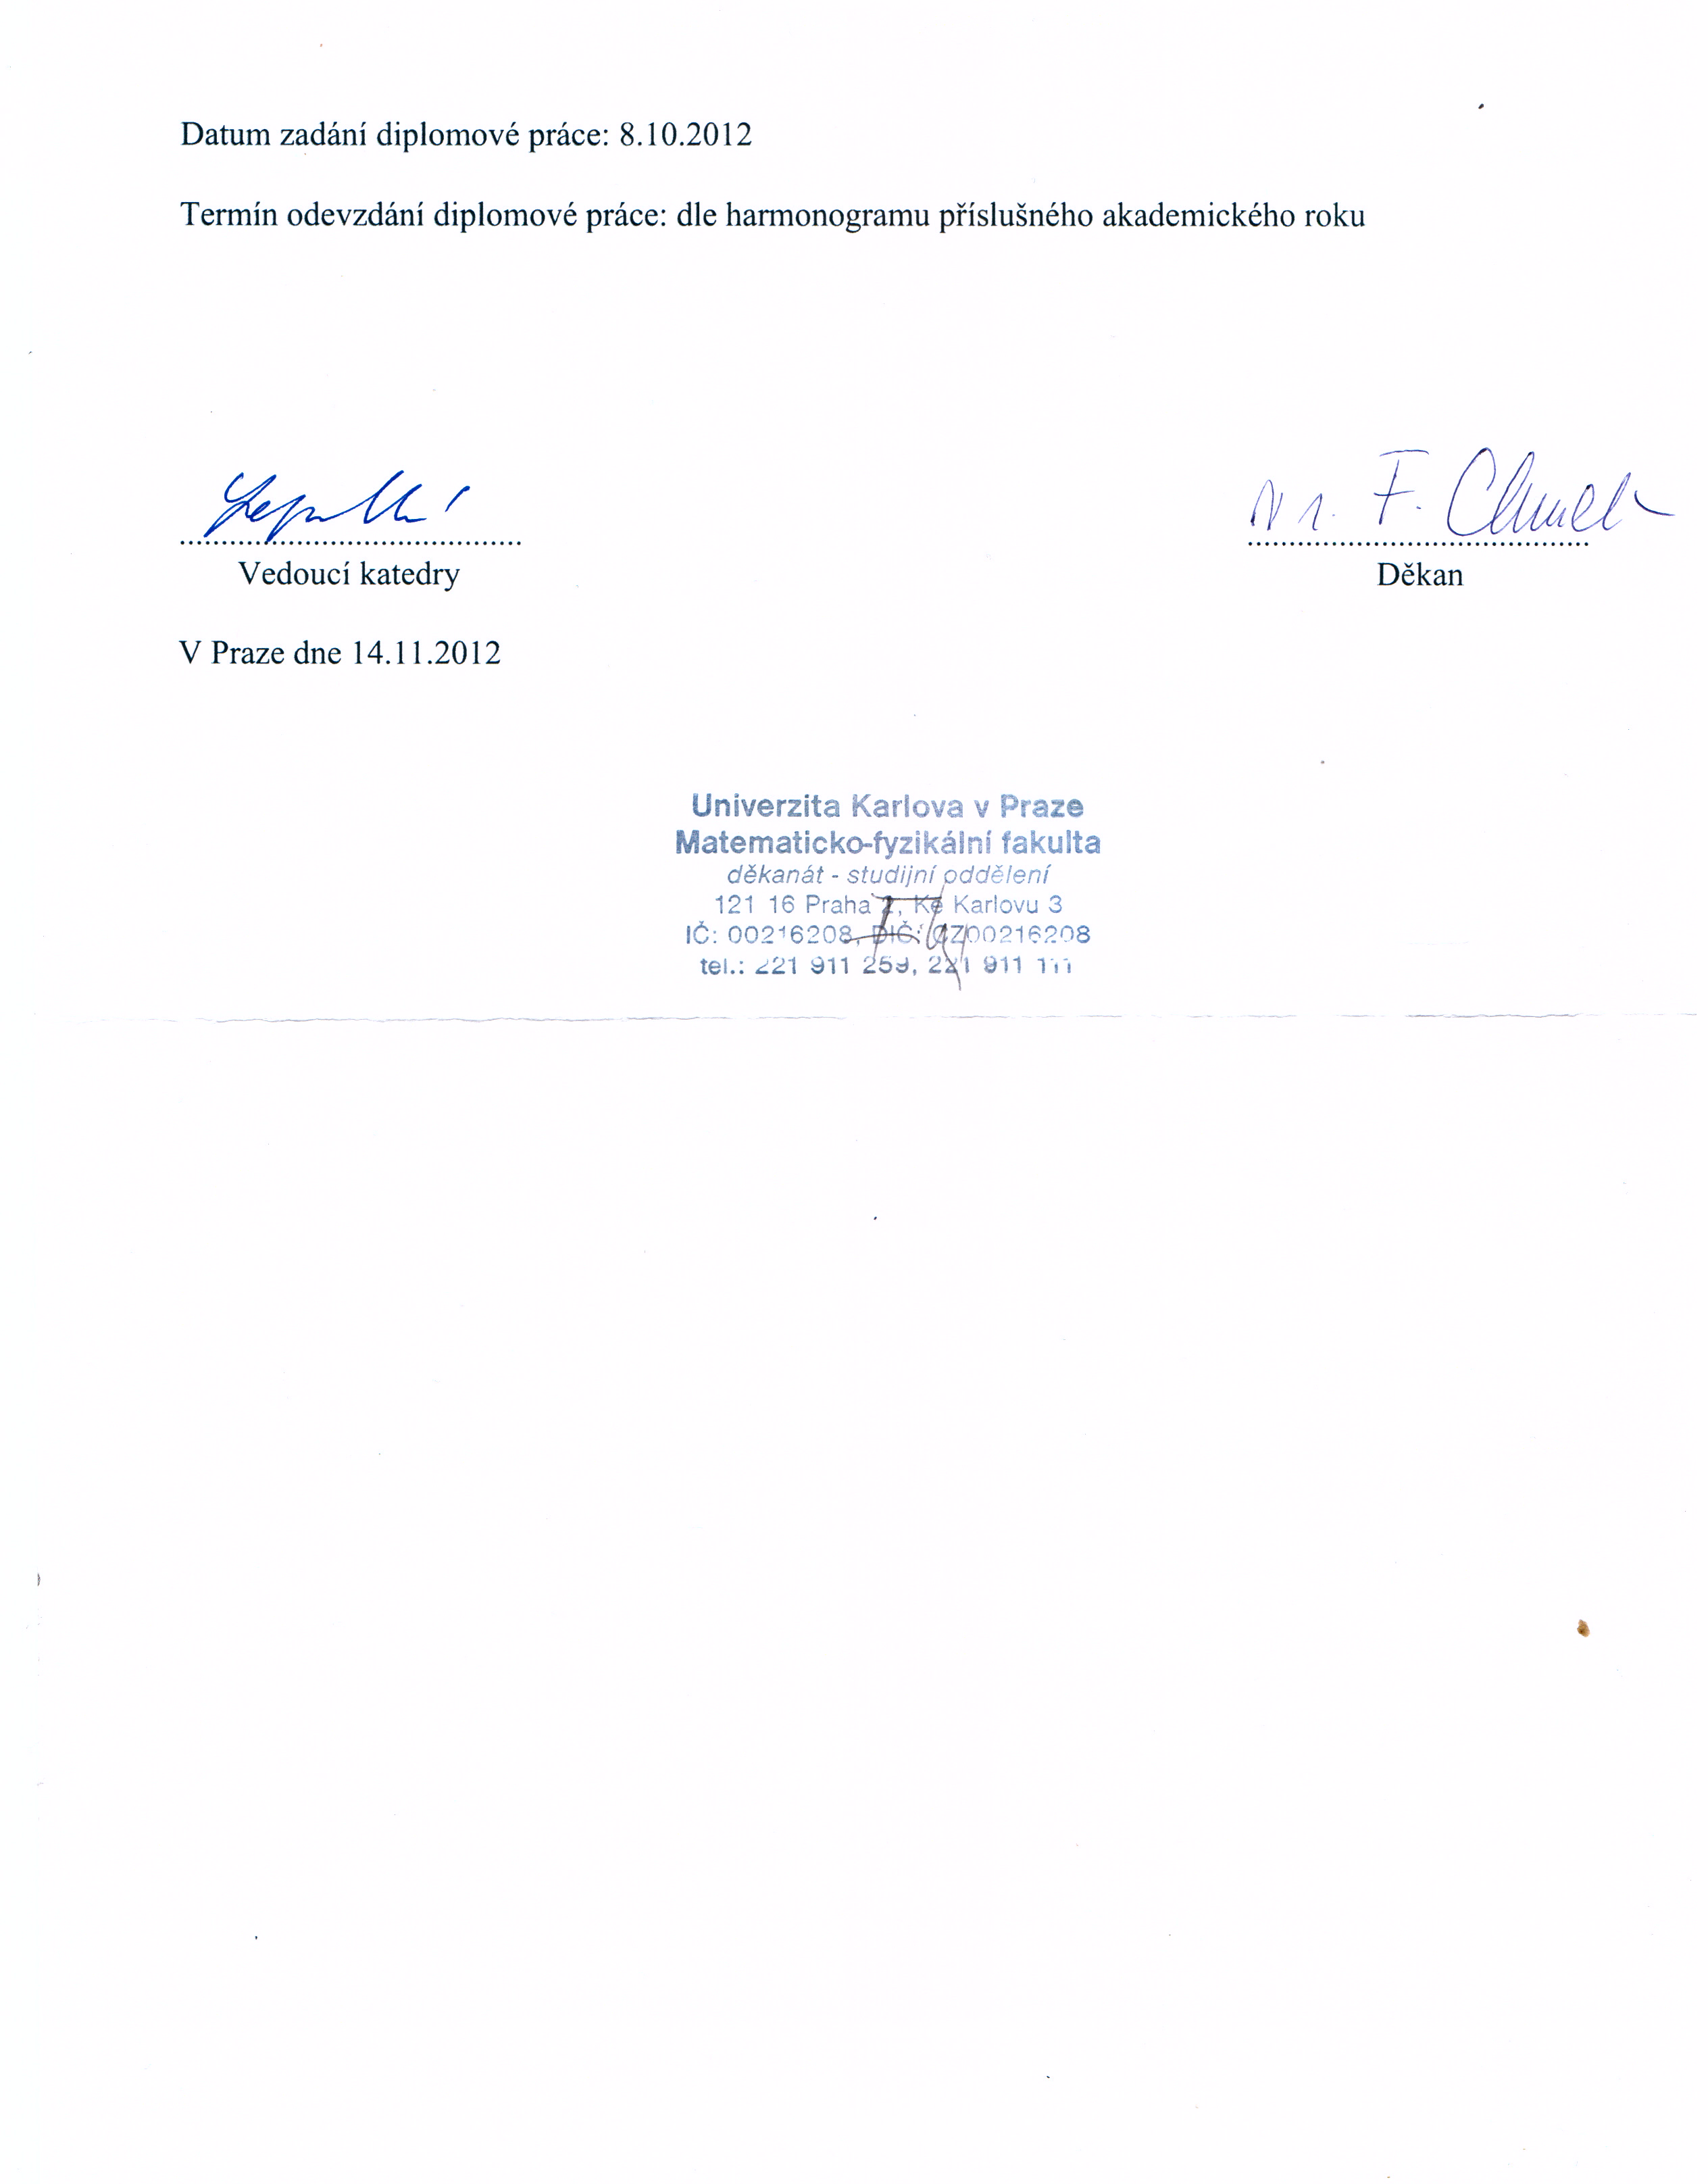
\includegraphics[scale=0.82]{zadani2}}
\end{figure}  

\newpage
%%%%%%%% end 2-3 page with master thesis task

%%% 4.(2.) title page
\normalsize % nastavení normální velikosti fontu
\vspace{10mm} 

\noindent I would like to thank my~supervisor, Ing. Mgr. Filip Jurčíček, Ph.D., for his advice, guidence and 
for keeping me motivated. 
I would like to thank namely, Matěj Korvas for HTK scripts results and advice, 
Lukáš Žilka, David Marek and Ondřej Dušek for hacks in Vim, Bash and Perl, 
Marek Vašut for advice with shared library linking, Tomáš Martinec for C++ advice
and Pavel Mencl for proofreading.
I am also very grateful to the~Kaldi team, which was very responsive and helpful.
Expecially, Daniel Povey and  Vassil Panayotov. 
Last but not least, I would like to thank my~parents and Adéla Čiháková for all the~help and support.


\vspace{\fill} % nastavuje dynamické umístění následujícího textu do spodní části stránky
\medskip\noindent
I declare that I wrote my master thesis independently and exclusively with~the~use of~the~cited sources. I agree with~lending and publishing this thesis.

I understand that my work relates to the~rights and obligations under the~Act No. 121/2000 Coll., the~Copyright Act, as amended, in particular the~fact that the~Charles University in Prague has the~right to conclude a~license agreement on the~use of~this work as a~school work pursuant to Section 60 paragraph 1 of~the~Copyright Act.

\noindent Prague, August 1, 2013 \hspace{\fill}Ondřej Plátek 

%%%   Výtisk pak na tomto míst+ nezapomente PODEPSAT!
%%%                                         *********

\newpage

%%% Následuje strana s abstrakty. Doplnte vlastní údaje.
\vbox to 0.5\vsize{
\setlength\parindent{0mm}
\setlength\parskip{5mm}
Název práce: Rozpoznávání řeči pomocí Kaldi\\
Autor: Ondřej Plátek\\
Katedra: Ústav formální a~aplikované lingvistiky\\
Vedoucí diplomové práce: Ing. Mgr. Filip Jurčíček, Ph.D.\\
E-mail vedoucího: jurcicek@ufal.mff.cuni.cz\\

\noindent Abstrakt:
Tématem této práce je implementace výkonného rozpoznávače v open-source systému trénování ASR~Kaldi~(\href{http://kaldi.sourceforge.net/}{http://kaldi.sourceforge.net/}) pro dialogové systémy. Kaldi již obsahuje ASR dekodéry, které však nejsou vhodné pro dialogové systémy. 
Hlavními důvody jsou jejich malá optimalizace na rychlost a~jejich velké zpoždění v generování výsledku po ukončení promluvy. 
Cílem této práce je proto vyvinutí real-time rozpoznávače pro dialogové systémy optimalizovaného na rychlost a minimalizujícího zpoždění.
     Zrychlení může být realizováno například pomocí multi-vláknového dekódování nebo s~využitím grafických karet pro obecné výpočty. 
 Součástí práce je také příprava akustického modelu a testování ve vyvíjeném dialogovém systému ”Vystadial”.


\noindent Klíčová slova: ASR,rozpoznávání mluvené řeči, dekodér

\vspace{10mm}

\noindent
Title: Automatic speech recognition using Kaldi\\
Author: Ondřej Plátek\\
Department: Ústav formální a aplikované lingvistiky \\
Supervisor: Ing. Mgr. Filip Jurčíček, Ph.D.\\
Supervisor's e-mail address: jurcicek@ufal.mff.cuni.cz\\

\noindent Abstract: 
The~topic of~this thesis is to implement efficient decoder for speech recognition 
training system ASR~Kaldi~(\href{http://kaldi.sourceforge.net/}{http://kaldi.sourceforge.net/}). 
Kaldi is already deployed with decoders, but they are not convenient for dialogue systems. 
The~main goal of~this thesis to develop a~real-time decoder for a~dialogue system, 
which minimize latency and optimize speed. Methods used for speeding up the~decoder are not 
limited to multi-threading decoding or usage of~GPU cards for general computations. 
Part of~this work is devoted to training an acoustic model and also testing it in the~"Vystadial" dialogue system.

\noindent Keywords: ASR,speech recognition, decoder

\vss}

\newpage

\openright
\pagestyle{plain}
\pagenumbering{arabic}
\setcounter{page}{1}
 
% % !TEX root = main.tex
\code{My Python Snippet}{Python}{snippets/test.py}
\code{My C Snippet}{C}{snippets/test.c}

\begin{figure}
    \begin{center}
    % Generated with LaTeXDraw 2.0.8
% Sun Mar 31 15:28:25 CEST 2013
% test coment
% \usepackage[usenames,dvipsnames]{pstricks}
% \usepackage{epsfig}
% \usepackage{pst-grad} % For gradients
% \usepackage{pst-plot} % For axes
\begin{figure}
\scalebox{1} % Change this value to rescale the drawing.
{
\begin{pspicture}(0,-1.4475)(6.685,1.5525)
\pscustom[linewidth=0.04]
{
\newpath
\moveto(5.74,1.0375)
\lineto(6.28,0.7475)
\curveto(6.55,0.6025)(6.665,0.1875)(6.51,-0.0825)
\curveto(6.355,-0.3525)(5.9,-0.5375)(5.6,-0.4525)
\curveto(5.3,-0.3675)(4.82,-0.1375)(4.64,0.0075)
\curveto(4.46,0.1525)(4.405,0.4625)(4.53,0.6275)
\curveto(4.655,0.7925)(4.945,1.0175)(5.11,1.0775)
\curveto(5.275,1.1375)(5.515,1.1825)(5.59,1.1675)
\curveto(5.665,1.1525)(5.755,1.1125)(5.8,1.0375)
}
\pscustom[linewidth=0.04]
{
\newpath
\moveto(5.16,1.1575)
\lineto(4.97,1.4075)
\curveto(4.875,1.5325)(4.76,1.4625)(4.7,0.8775)
}
\pscustom[linewidth=0.04]
{
\newpath
\moveto(5.82,1.0575)
\lineto(6.04,1.2375)
\curveto(6.15,1.3275)(6.25,1.2825)(6.22,0.8775)
}
\pscustom[linewidth=0.04]
{
\newpath
\moveto(5.32,0.4175)
\lineto(5.44,0.3575)
\curveto(5.5,0.3275)(5.525,0.3075)(5.42,0.3375)
}
\pscustom[linewidth=0.04]
{
\newpath
\moveto(5.36,0.4175)
\lineto(5.53,0.3875)
\curveto(5.615,0.3725)(5.62,0.3975)(5.54,0.4375)
}
\pscustom[linewidth=0.04]
{
\newpath
\moveto(5.94,0.6175)
\lineto(6.13,0.6075)
\curveto(6.225,0.6025)(6.22,0.5625)(6.12,0.5275)
\curveto(6.02,0.4925)(5.915,0.4575)(5.9,0.4575)
}
\pscustom[linewidth=0.04]
{
\newpath
\moveto(4.46,0.6575)
\lineto(3.64,0.8975)
\curveto(3.23,1.0175)(2.56,0.7825)(2.3,0.4275)
\curveto(2.04,0.0725)(1.98,-0.3725)(2.18,-0.4625)
\curveto(2.38,-0.5525)(2.94,-0.6775)(3.3,-0.7125)
\curveto(3.66,-0.7475)(4.17,-0.6425)(4.32,-0.5025)
\curveto(4.47,-0.3625)(4.68,-0.1725)(4.74,-0.1225)
}
\pscustom[linewidth=0.04]
{
\newpath
\moveto(4.52,-0.4625)
\lineto(4.81,-0.6425)
}
\pscustom[linewidth=0.04]
{
\newpath
\moveto(4.28,-0.7025)
\lineto(4.76,-0.8625)
}
\pscustom[linewidth=0.04]
{
\newpath
\moveto(2.1,-0.0625)
\lineto(1.31,-0.2025)
\curveto(0.915,-0.2725)(0.305,-0.1575)(0.09,0.0275)
\curveto(-0.125,0.2125)(-0.17,0.3925)(0.0,0.3875)
\curveto(0.17,0.3825)(0.525,0.2875)(0.71,0.1975)
\curveto(0.895,0.1075)(1.265,0.0375)(1.45,0.0575)
\curveto(1.635,0.0775)(1.875,0.0875)(2.04,0.0575)
}
\usefont{T1}{ptm}{m}{n}
\rput(4.342656,-1.2925){Kocka domaci}
\end{pspicture} 
}
\label{label-kocka}
\caption{Caption - kocka}
\end{figure}


    \caption{Test kocka}
    \label{pic:kocka} 
    \end{center}
\end{figure}


\ac{BW}

% {{{
Lorem ipsum dolor sit amet, consetetur sadipscing elitr, sed diam nonumy eirmod
tempor invidunt ut labore et dolore magna aliquyam erat, sed diam voluptua. At
\ml{Did you know Lorem Ipsum before?}
vero eos et accusam et justo duo dolores et ea rebum. Stet clita kasd gubergren,
no sea takimata sanctus est Lorem ipsum dolor sit amet.
% }}}

What the \ac{ARPA} hack is it?

% !TEX root = main.tex
\chapter{Introduction}
\label{chap:intro}

% todo few words
% 
% stezejni integrace - dialogovy system
%     jedna~cesta~OpenJulius - one-best OK, lattice malo kvalitni
% 
% srovnani OpenJulius
%     Kdo dela~lepsi lattice
%     kouknout se na~OpenJulius scripty
%     a~porovnat je
% 
% uvolneni: Budou volne dostupny a~pak clanek a~tutorial
% o datech o trenovacich sktriptech a~o decodovani pres 2 jazyky

A spoken dialog is the most intuitive way of~communication among people. Nowadays, the spoken dialog is becoming popular choice of~communication even for human-device interaction. The quality of~a~dialog largely depends on the quality of~speech recognition, because the~reasoning and the~reply is based on the recognized speech. 

In this work, we hope to improve speech recognition in the dialog system developed at UFAL MFF UK, called Alex. One of~the application of~our dialog system Alex is a~public phone call service, where a~user can ask Alex about navigation in Prague public transport.

\section{The problem} 
\label{sec:why}
The Alex dialog system and this thesis was partly funded by the Ministry of~Education, Youth and Sports
of~the Czech Republic under the grant agreement LK11221 for~the~{\it Vystadial project}\/ and core research of~Charles University in Prague.
Let us cite the main goals of~the~{\it Vystadial project}\cite{jurcicek2012vystadial}:
\begin{quote}
    \begin{itemize}
        \item Study and improve methods for learning of~statistical models used in dialogue systems. 
        \item Create software infrastructure for remote training and evaluation.
        \item Release the developed dialogue system under open-source license.
        \item Create publicly available corpus of~audio recordings, transcriptions and semantic annotations for training dialogue systems.
    \end{itemize}
\end{quote}

The Alex dialog system has been using the HTK toolkit\cite{young94htk} to train acoustic models and the OpenJulius\cite{lee2009julius} decoder for real time decoding. Nevertheless, the used set up has several flaws.

One of~our main goals is to release the Alex dialog system under Apache License, Version 2.0\footnote{\url{http://www.apache.org/licenses/LICENSE-2.0}}, which is very permissive for users. On the other hand, the HTK toolkit uses quite restrictive license. The license does not allow us to change the source code of~its decoders (HDecode and HVite) and release the changed code under Apache license. 

Without a~source code modification interfacing the decoder from our dialog system is difficult. In addition, we need to implement specific output formats for speech recognition in order to improve the Alex dialog system.

The other decoder used in Alex is the~OpenJulius decoder, which is released under revised BSD style license. This license is much better from our point of~view. On the other hand, we have experienced software instability using OpenJulius decoder. In addition, OpenJulius seems to be hard to be patched or otherwise improved due to its coding style. Currently, it seems, that the stability problems around OpenJulius are not going to be resolved in near feature.

The Kaldi\cite{povey2011kaldi} framework solves the drawbacks of~HTK and OpenJulius. It is released under Apache License, Version 2.0. The same license we want to use. The Kaldi framework is cleanly written and has a~responsive developer community. The decoders implemented in Kaldi already support lattices and confusion networks generation. Currently, the Kaldi framework is mostly used for experimenting and it is not meant for real time usage. However, in August 2012\footnote{The changes were introduced by \href{https://sourceforge.net/p/kaldi/code/1259/}{svn commit 1259}.} Kaldi team published a~testing version of~an online decoder. In this thesis we hope to improve and integrate the online decoder into Alex dialog system for a~real time use.

% section why_introducing_new_decoder_and_toolkit_for_training_acoustic_models_ (end)

\section{The goals of~the~thesis} 
\label{sec:goals}
Let us introduce the goals of~this thesis. Each of~the~goals is described in one of subsections below. Note, that the goals are described in top down approach.
At first, we introduce the goal of integration the final real-time decoder into our~dialog system, and later we specify subgoals needed for the integration.
At~last, we promise to evaluate the work done.

\subsection{A~real-time decoder integration} 
\label{sub:integration}
The Alex dialog system is developed in Python language and consist of~six major components. 
\begin{enumerate}
    \item Voice Activity Detection (VAD)
    \item Automatic Speech Recognition (ASR) 
    \item Spoken Language Understanding (SLU)
    \item Dialog Manager (DM)
    \item Natural Language Generation (NLG)
    \item Text To Speech (TTS)
\end{enumerate}
The~Alex dialog system has a~speech to speech user interface. The~system interacts with the user in {\it turns}. During a~single turn the dialog system waits for a~user spoken input, process the speech and generates the reply.
The~data~flow during single turn is depicted in~Figure~\ref{fig:dialog_system}.

The integration task consist of:
\begin{itemize}
    \item Building a~Python interface for a~C++ Kaldi decoder.
    \item Define the input and output interface for the Kaldi decoder - wrapped by Automatic Speech Recognition (ASR) unit in Alex.
\end{itemize}
 The ASR unit takes output of~the VAD component and provides input for the SLU unit. 
 %The input and output interfaces are chosen according the real time needs of~the VAD unit and the SLU unit.

\begin{figure}
    \begin{center}
    % Generated with LaTeXDraw 2.0.5
% Wed Apr 09 16:50:40 CEST 2014
% \usepackage[usenames,dvipsnames]{pstricks}
% \usepackage{epsfig}
% \usepackage{pst-grad} % For gradients
% \usepackage{pst-plot} % For axes
\scalebox{1} % Change this value to rescale the drawing.
{
\begin{pspicture}(0,-3.66)(14.64,3.66)
\definecolor{color685}{rgb}{0.11764705882352941,0.14901960784313725,0.8901960784313725}
\definecolor{color523}{rgb}{0.027450980392156862,0.25882352941176473,0.8431372549019608}
\definecolor{color34}{rgb}{0.7843137254901961,0.0784313725490196,0.23529411764705882}
\psellipse[linewidth=0.04,dimen=outer](5.55,1.51)(0.83,0.69)
\usefont{T1}{ptm}{m}{n}
\rput(5.5046873,1.425){VAD}
\psellipse[linewidth=0.04,dimen=outer](8.97,2.61)(0.83,0.69)
\usefont{T1}{ptm}{m}{n}
\rput(8.942186,2.525){ASR}
\psellipse[linewidth=0.04,dimen=outer](12.51,1.15)(0.83,0.69)
\usefont{T1}{ptm}{m}{n}
\rput(12.455312,1.065){SLU}
\psellipse[linewidth=0.04,dimen=outer](12.61,-1.51)(0.83,0.69)
\usefont{T1}{ptm}{m}{n}
\rput(12.567813,-1.595){DM}
\psellipse[linewidth=0.04,dimen=outer](5.49,-1.27)(0.83,0.69)
\usefont{T1}{ptm}{m}{n}
\rput(9.001249,-2.315){NLG}
\psellipse[linewidth=0.04,dimen=outer](9.03,0.0)(5.61,3.66)
\usefont{T1}{ptm}{m}{n}
\rput(5.4315624,-1.355){TTS}
\psellipse[linewidth=0.04,dimen=outer](9.03,-2.23)(0.83,0.69)
\usefont{T1}{ptm}{m}{n}
\rput(9.0,0.24){\Huge Dialogue System}
\psline[linewidth=0.04cm,arrowsize=0.05291667cm 2.0,arrowlength=1.4,arrowinset=0.4]{->}(9.76,2.38)(11.9,1.6)
\psline[linewidth=0.04cm,arrowsize=0.05291667cm 2.0,arrowlength=1.4,arrowinset=0.4]{->}(6.36,1.76)(8.18,2.42)
\psline[linewidth=0.04cm,arrowsize=0.05291667cm 2.0,arrowlength=1.4,arrowinset=0.4]{->}(12.54,0.46)(12.56,-0.86)
\psline[linewidth=0.04cm,arrowsize=0.05291667cm 2.0,arrowlength=1.4,arrowinset=0.4]{->}(11.84,-1.74)(9.9,-2.32)
\psline[linewidth=0.04cm,arrowsize=0.05291667cm 2.0,arrowlength=1.4,arrowinset=0.4]{->}(8.14,-2.18)(6.3,-1.52)
\pscircle[linewidth=0.04,dimen=outer](0.98404694,2.1548762){0.6451238}
\psline[linewidth=0.04cm](1.0,1.0)(0.92,-0.16)
\psline[linewidth=0.04cm](0.98193634,1.0577894)(0.0,1.84)
\psline[linewidth=0.04cm](0.98193634,1.0432783)(2.0694895,2.1461184)
\psline[linewidth=0.04cm](0.9072397,-0.23489322)(1.46,-1.72)
\psline[linewidth=0.1cm,linecolor=color523,linestyle=dashed,dash=0.16cm 0.16cm,arrowsize=0.05291667cm 2.0,arrowlength=1.4,arrowinset=0.4]{->}(2.28,1.86)(4.46,1.5)
\psline[linewidth=0.1cm,linecolor=color523,linestyle=dashed,dash=0.16cm 0.16cm,arrowsize=0.05291667cm 2.0,arrowlength=1.4,arrowinset=0.4]{<-}(2.32,-0.52)(4.36,-0.88)
\usefont{T1}{ptm}{m}{n}
\rput(3.0603125,-1.055){\Large \color{color685}Speech}
\usefont{T1}{ptm}{m}{n}
\rput(3.0803125,1.345){\Large \color{color685}Speech}
\usefont{T1}{ptm}{m}{n}
\rput(6.8231244,2.605){\color{color34}Speech}
\usefont{T1}{ptm}{m}{n}
\rput(11.20875,2.605){\color{color34}Text/Lattice}
\usefont{T1}{ptm}{m}{n}
\rput(12.445,-0.435){\color{color34}Semantic meaning}
\usefont{T1}{ptm}{m}{n}
\rput(11.265624,-2.255){\color{color34}Action}
\usefont{T1}{ptm}{m}{n}
\rput(6.899688,-2.175){\color{color34}Text}
\psline[linewidth=0.04cm](0.8872397,-0.23489322)(0.1,-1.62)
\psline[linewidth=0.04cm](0.36193633,2.0032785)(1.72,2.76)
\psdots[dotsize=0.12](1.34,2.28)
\rput{48.07518}(1.8088533,-0.49558815){\psarc[linewidth=0.04](1.46,1.78){0.12}{0.0}{180.0}}
\psline[linewidth=0.04cm](1.0368464,1.4389827)(1.0031536,1.1610173)
\end{pspicture} 
}

    \caption{Single turn in Alex dialog system}
    \label{fig:dialog_system} 
    \end{center}
\end{figure}

In our dialog system we experiment with different outputs of~a~speech decoder in Spoken Language Understanding unit. 
The decoder for our system should be able to generate {\it n-best lists}, {\it lattices} and {\it confusion networks} output.
% Ideally, the decoder for our system would be able to generate {\it n-best lists}, {\it lattices} and {\it confusion networks}.

%   d) output of~the decoder will be standard lattices 
%     (both phone and word)
%   e) compute posterior lattices (both phone and word),
%   f) provide confusion networks for these lattices
%   g) measure teh quality of~the lattices, depth, oracle error rate    

% section integrate_kaldi_decoder_into_vystadial_framework (end)


\subsection{Development of~a~real time decoder}
\label{sub:kaldi_rt_decoder}
In the our dialog system we need above all a~real time decoder for the Kaldi toolkit. At first, we will identify what prevents the current KALDI decoders from being used as real time decoders. 

Namely, we will explore problems with latency and suggest potential speed improvements e.g.\ approximations, use of~GPU, and so on. Based on the experiments we will suggest the optimal setting for the real time use of~Kaldi decoder.

% section development_of_real_time_asr_decoder_for_the_kaldi_toolkit (end)

\subsection{Training acoustic models and a~language model} 
\label{sub:training_kaldi_acoustic_models}
Every modern continuous speech recognition engine requires two pre trained components, an~acoustic model and a~language model. We will focus on finding the best acoustic model for the~Kaldi toolkit. We will use a basic language model, because we want to compare HTK and Kaldi toolkit acoustic models accuracy.  In addition, we can reuse the already built language model for HTK. Other reason is that a language model is very domain dependent. % FIXME add citation LM are domain dependent
We want to use our Alex dialog system in other domains except Prague public transport, so we do not focus on language modeling. 

We have been using the HTK acoustic models together with OpenJulius and HTK decoders. We will develop training scripts for acoustic models using Kaldi toolkit. The acoustic models will be evaluated using different Kaldi decoders and the same language model as used in HTK training scripts. 

During the phase of~training acoustic models, we focus mainly on the quality of~the decoded output rather than on the speed of~decoding itself. 
% We would like to achieve at least as accurate decoding with Kaldi acoustic models as we have achieved with HTK models. In this thesis we will set up and evaluate following experiments using Kaldi:
We would like to achieve at least as accurate decoding with Kaldi as we have achieved with HTK. In this thesis we will set up and evaluate following experiments using Kaldi:
\begin{itemize}
    \item Standard generative training
    \item Learning linear transformations (e.g. HLDA\footnote{The abbreviation HLDA stands for heteroscedastic linear discriminant analysis.})
    \item Discriminative training 
\end{itemize}
% section training_kaldi_acoustic_models (end)
 

\subsection{Evaluating decoders} 
\label{sub:compare_rt}
After training acoustic models with~sufficient quality we will balance accuracy and speed for the Kaldi online decoder. Trading decoding speed for a speech recognition accuracy is common technique for speeding up decoders and can be applied on all decoders of interests. We will evaluate following decoders:
\begin{itemize}
    \item HVite  % FIXME test this through Subprocess
    \item HDecode % FIXME test this through Subprocess
    \item OpenJulius % FIXME test this through Subprocess/Sockets
    \item Kaldi decoders
    \item Improved online Kaldi decoder
\end{itemize}

The speed of~the decoders will be expressed in terms of~real time factor.\footnote{Real time factor $RTF$ is metric for comparing speed of~decoders. It is defined as $RTF = \frac{P}{D}$, where $P$ is time of~the processing the audio by a~decoder on input with length $D$.} The accuracy will be expressed in terms of~word error rate (WER).

We will also compare and contrast possibilities of~different output formats for each of~tested decoders. The~memory consumption and the~stability of~decoders will be also observed. 

% section compare_real_time_abilities_of_already_used_and_kaldi_decoders (end)

% section goals (end)

\section{Outline of~the thesis} 
\label{sec:outline_of_the_thesis}
In~Chapter~\ref{cha:background} we introduce speech recognition algorithms. At first we introduce standard algorithms. Later, we focus on Finite State Automata~framework used by Kaldi. In~Chapter~\ref{cha:training} we describe how we trained the acoustic models needed by Kaldi decoder. In addition, we shortly contrast and compare training methods in HTK and Kaldi. Chapter~\ref{cha:decoder} presents the Kaldi real time decoder embedded into our dialog system. We discuss the architecture of~the decoder, its properties. We also distinguish what is the original work done by Kaldi team and what are our improvements. At the end of~Chapter~\ref{cha:decoder} we describe the qualities of~the developed decoder and compare it with other decoders used in our dialog system.
The~Chapter~\ref{cha:integration} explains how we integrated C++ decoder in our dialog system written in Python.
    
The speech recognition algorithms described in~Chapter~\ref{cha:background} are meant like short introduction to the~problematic, which allow readers understand next chapters. The~Chapter~\ref{cha:training} explains that Kaldi framework is capable of~training acoustic models and decoding with them with no worse accuracy than HTK toolkit. In~Chapter~\ref{cha:integration} we discuss technical difficulties related with integration. 

Finally, the~Chapter~\ref{cha:conclusion} summarises the thesis and finishes with future research directions.

% section outline_of_the_thesis (end)

\chapter{Goals}
\label{cha:goals}
This chapters describes the goals of this thesis. 
In addition, in~Section~\ref{sec:why} we explain the objectives for integrating Kaldi framework into the dialog system Vystadial.\footnote{Vystadial is spoken dialogue system internally developed at UFAL MFF.} 

\section{Development of real time ASR decoder for the Kaldi toolkit}\footnote{The abbreviation ASR stands for automatic speech recognition.} 
\label{sec:development_of_real_time_asr_decoder_for_the_kaldi_toolkit}
Our main goal is is to develop a real time ASR decoder for the Kaldi toolkit. At first, we will identify what prevents the current KALDI decoders from being used as real time decoders. Namely, we will explore problems with latency and suggest potential speed improvements e.g. approximations, use of GPU, and so on. Based on the experiments we will suggest the optimal setting for the real time use of Kaldi decoder.

% section development_of_real_time_asr_decoder_for_the_kaldi_toolkit (end)

\section{Training Kaldi acoustic models} 
\label{sec:training_kaldi_acoustic_models}
Well trained models together with real time decoder recognize speech fast and with desired quality.

In the Vystadial project we have so far used HTK acoustic models with different decoders.
We want to develop training scripts for Kaldi framework which will produce acoustic models used with Kaldi decoders. The quality of the output for the Kaldi acoustic models and decoders should be better or comparable with~the~output of~acoustic models trained by HTK scripts and used against HDecode and OpenJulius decoders.

Using the Kaldi framework we will perform experiments which implement:
\begin{itemize}
    \item Standard generative training
    \item Learning linear transformations (e.g. HLDA\footnote{The abbreviation HLDA stands for heteroscedastic linear discriminant analysis})
    \item Discriminative training 
\end{itemize}

% section training_kaldi_acoustic_models (end)
 

\section{Comparison of used decoders and Kaldi decoders} 
\label{sec:compare_real_time_abilities_of_already_used_and_kaldi_decoders}
The main stress will be in comparing real time abilities and accuracy.
The speed of the decoders will be expressed in terms of real time factor.
The accuracy will be expressed in terms of word error rate (WER).

We will also compare and contrast possibilities of different output formats for each of tested decoders.
In addition we will take into account the memory consumption and stability of decoders.

There are HVite, HDecode, OpenJulius and Kaldi decoders to be evaluated.
% section compare_real_time_abilities_of_already_used_and_kaldi_decoders (end)

\section{Integrate Kaldi decoder into Vystadial framework} 
\label{sec:integrate_kaldi_decoder_into_vystadial_framework}
The Vystadial project is developed in Python language and consist of five major components.
The dialog system provides speech to speech interface. The components are linked into pipeline in order to process the spoken input and to generate speech.
Pipeline consist of:
\begin{enumerate}
    \item Voice Activity Detection (VAD)
    \item Automatic Speech Recognition (ASR) - Here we run one of our decoders.
    \item Semantic and Language Analysis (SLU)
    \item Dialog Manager (DM)
    \item Natural Language Generation (NLG)
\end{enumerate}

The integration task consist of building the Python interface for C++ Kaldi decoders and define the input and output interface for the ASR unit. We consider the VAD unit to be finished and we will not change it. Consequently, the input interface for ASR unit will be the same for all experiments. On the other hand, we need to create several interfaces and among ASR and SLU units according type of ASR output.

The reason for different ASR outputs is given by the needs of SLU unit. The SLU unit may work better with word lattices or confusion networks instead of classical textual ASR output. In this thesis we aim at providing different interfaces to SLU unit without any further experiments.

% 5) Implement RT decoder for KALDI (this will be C/C++), 
%   a) also implement integration with Python
%   b) perform optimisation of the code and the methods, 
%     especially make sure that you minimise the latency 
%     between the end of utterance and the returned results
%   c) use GPU for computing observation probabilities (GPU labeler), 
%     however, make sure that the GPU is not required
%   d) output of the decoder will be standard lattices 
%     (both phone and word)
%   e) compute posterior lattices (both phone and word),
%   f) provide confusion networks for these lattices
%   g) measure teh quality of the lattices, depth, oracle error rate    

% section integrate_kaldi_decoder_into_vystadial_framework (end)

    
\section{Why introducing a new decoder and toolkit for training acoustic models?} 
\label{sec:why}
In previous sections we introduced the goals of this thesis. In this section we argue why is the work necessary at all.


% section why_introducing_new_decoder_and_toolkit_for_training_acoustic_models_ (end)



So far, the Vystadial project is using the HTK toolkit to train acoustic models and the OpenJulius ASR for real time decoding.
% chapter goals (end)

\subsection{Kaldi Experiment Results} % (fold)
\label{sub:Experiment results}

Corresponding HTK results could be found at
\href{https://redmine.ms.mff.cuni.cz/projects/vystadial/wiki/Acoustic_models/} {Vystadial Redmine Wiki}


{\bf RT coef = Minimum over number of jobs for each tasks
WER, SER = Minimum over iterations 9-20 of rescoring for each tasks, 
(The iterations for WER(SER) minimum is the second number in the brackets)}


1. experiment kaldi-vystadial-recipe commit cf40202263450c72b4f8ef9aa8d6b7f03ac59814\\
Data classic

\begin{tabular}{cccc}
exp             & RT coef        & WER         & SER        \\
tri2b-mpe       & 0.88688125     & (23.54, 20) & (51.73, 20)\\
mono            & 3.2617725      & (50.3, 20)  & (75.07, 20)\\
tri3b-mmi       & 0.807879083333 & (22.73, 19) & (50.53, 15)\\
tri1            & 1.94605        & (33.34, 20) & (66.4, 20) \\
tri3b-denlats   & 0.77643725     & None        & None       \\
tri2b-mmi       & 1.72681375     & (23.03, 15) & (50.8, 20) \\
tri2a           & 1.962175       & (33.19, 20) & (66.0, 20) \\
tri2b           & 1.8105575      & (30.08, 19) & (63.47, 19)\\
tri3b           & 0.748003125    & (31.37, 19) & (63.47, 19)\\
tri3b-fmmi-c    & 11.8128208333  & (22.24, 16) & (49.2, 15) \\
tri3b-fmmi-b    & 8.22911708333  & (21.67, 17) & (48.27, 14)\\
tri2b-mmi-b0.05 & 1.146794625    & (22.29, 17) & (49.87, 17)\\
tri2b-denlats   & 1.02629525     & None        & None       \\
tri3b-fmmi-d    & 6.60894458333  & (22.51, 18) & (49.6, 15)
\end{tabular}


2. experiment kaldi-vystadial-recipe commit 10fe1128519aa263ab805216e381d15378d74821\\
Data classic

\begin{tabular}{cccc}
exp             & RT coef       & WER         & SER        \\
-ri3b-fmmi-b    & 10.422085     & (19.64, 14) & (45.07, 11)\\
tri2b-mpe       & 2.09137125    & (22.06, 15) & (49.6, 14) \\
mono            & 3.4773675     & (48.69, 18) & (74.4, 18) \\
tri3b-mmi       & 1.25892633333 & (20.11, 18) & (47.73, 11)\\
tri1            & 4.459925      & (26.92, 16) & (56.27, 20)\\
tri3b-denlats   & 1.2851525     & None        & None       \\
tri2b-mmi       & 1.68427875    & (20.88, 17) & (46.67, 14)\\
tri2a           & 2.3842725     & (26.09, 17) & (55.07, 17)\\
tri2b           & 1.7085825     & (26.16, 20) & (57.73, 20)\\
tri3b           & 1.073698375   & (27.57, 20) & (58.8, 16) \\
tri3b-fmmi-c    & 12.1484916667 & (19.52, 15) & (45.47, 11)\\
tri2b-mmi-b0.05 & 1.79180375    & (20.63, 14) & (46.4, 14) \\
tri2b-denlats   & 1.196845      & None        & None       \\
tri3b-fmmi-d    & 9.047925      & (19.42, 15) & (45.07, 12)
\end{tabular}


3. experiment kaldi-vystadial-recipe commit 585de385922b431881dfd2508567917045a104ab\\
Data vystadial
CHEATING: TEST DATA ARE SUBSET OF TRAIN DATA
on data /ha/projects/vystadial/data/asr/en/voip/{train.old, test.old}

\begin{tabular}{cccc}
exp             & RT coef        & WER         & SER        \\
-ri3b-fmmi-b    & 8.49685875     & (11.32, 15) & (32.6, 20) \\
tri2b-mpe       & 1.042053       & (12.7, 19)  & (36.61, 19)\\
mono            & 2.46068        & (43.51, 13) & (64.17, 15)\\
tri3b-mmi       & 0.921234416667 & (12.21, 14) & (33.89, 18)\\
tri1            & 1.6237775      & (16.87, 19) & (43.73, 19)\\
tri3b-denlats   & 1.03578075     & None        & None       \\
tri2b-mmi       & 1.197875       & (11.52, 11) & (32.86, 17)\\
tri2a           & 1.5251075      & (17.09, 12) & (44.24, 19)\\
tri2b           & 1.060909       & (16.06, 20) & (43.08, 20)\\
tri3b           & 0.77341175     & (17.02, 17) & (44.11, 20)\\
tri3b-fmmi-c    & 8.77094958333  & (12.28, 16) & (34.02, 16)\\
tri2b-mmi-b0.05 & 1.119341       & (11.2, 16)  & (32.08, 17)\\
tri2b-denlats   & 0.9729795      & None        & None       \\
tri3b-fmmi-d    & 6.58549958333  & (11.86, 13) & (33.25, 12)
\end{tabular}


4. experiment kaldi-vystadial-recipe commit 585de385922b431881dfd2508567917045a104ab\\
Data vystadial (/ha/projects/vystadial/data/asr/en/voip/{train, test})

\begin{tabular}{cccc}
exp             & RT coef       & WER         & SER        \\
-ri3b-fmmi-b    & 10.5736754167 & (16.87, 16) & (40.62, 16)\\
tri2b-mpe       & 1.2229925     & (17.34, 14) & (41.53, 16)\\
mono            & 2.81766       & (41.59, 13) & (65.72, 15)\\
tri3b-mmi       & 1.07604041667 & (18.23, 14) & (42.69, 15)\\
tri1            & 2.12002       & (23.19, 18) & (50.97, 18)\\
tri3b-denlats   & 0.94768325    & None        & None       \\
tri2b-mmi       & 1.59091125    & (17.49, 14) & (41.27, 15)\\
tri2a           & 1.91198       & (21.44, 15) & (48.9, 15) \\
tri2b           & 1.54646       & (20.62, 18) & (48.38, 18)\\
tri3b           & 0.9433825     & (21.56, 17) & (52.13, 17)\\
tri3b-fmmi-c    & 11.175855     & (17.29, 14) & (41.27, 17)\\
tri2b-mmi-b0.05 & 1.5890125     & (17.22, 15) & (41.01, 15)\\
tri2b-denlats   & 1.00629875    & None        & None       \\
tri3b-fmmi-d    & 8.39958958333 & (16.9, 13)  & (40.62, 17)
\end{tabular}


5. experiment kaldi-vystadial commit 4e96c6704785b2476daf26e0b39eec95f3157f1e
Data vystadial (/ha/projects/vystadial/data/asr/en/voip/{train, test})
Removed OOV words from LM $\longrightarrow$ decoder is not trained for OOVs and does not produce
any symbol for OOV

\begin{tabular}{cccc}
exp             & RT coef       & WER         & SER        \\
-ri3b-fmmi-b    & 14.6555625    & (15.57, 19) & (37.9, 14) \\
tri2b-mpe       & 2.4290175     & (16.25, 16) & (41.4, 20) \\
mono            & 4.68498       & (43.02, 14) & (65.59, 13)\\
tri3b-mmi       & 2.5989        & (19.63, 20) & (46.57, 16)\\
tri1            & 4.00148       & (22.61, 18) & (50.84, 17)\\
tri3b-denlats   & 2.3944975     & None        & None       \\
tri2b-mmi       & 3.11491875    & (16.03, 18) & (41.27, 18)\\
tri2a           & 3.5336175     & (22.02, 15) & (49.55, 20)\\
tri2b           & 2.6743175     & (19.88, 20) & (47.48, 20)\\
tri3b           & 1.807084875   & (20.54, 17) & (47.22, 17)\\
tri3b-fmmi-c    & 14.7587791667 & (15.74, 15) & (38.03, 14)\\
tri2b-mmi-b0.05 & 3.23086       & (15.88, 17) & (40.88, 20)\\
tri2b-denlats   & 2.2504575     & None        & None       \\
tri3b-fmmi-d    & 10.4809795833 & (15.62, 14) & (38.03, 16)
\end{tabular}

\todo{FIND OUT IF ITERATIONS MATCHES ADDING ITERATIONS ADDING GAUSSIANS}

% subsection Experiment results (end)

\section{Kaldi Framework} % (fold)
\label{sec:Kaldi Framework}

\subsubsection*{Sources} % (fold)

\begin{itemize}
    \item \href{http://kaldi.sourceforge.net/graph.html} {Decoding graph construction in Kaldi}
    \item \href{http://kaldi.sourceforge.net/lattices.html} {Lattices in Kaldi}
\end{itemize}

\subsubsection*{Decoding graph construction} % (fold)
Kaldi uses Finite-State Transducers (FST) as underlaying representation for all models, which are used to decoding. Consequently, training and decoding of models in Kaldi can be expressed as sequence of operations above FSTs.

Decoding is performed using a final result of training, so called {\it decoding graph}. 
From the high level point of view,
during training we are constructing the decoding graph 
\begin{equation} \label{eq:hclg}
HCLG = H\circ C\circ L\circ G
\end{equation}.

The symbol $\circ$ represents an associative binary operation of composition on FST.
Namely, the transducers appearing in equation \ref{eq:hclg} are:
\begin{enumerate}
    % source  http://kaldi.sourceforge.net/graph.html
    \item G is an acceptor that encodes the grammar or language model.
    \item L is the lexicon. Its input symbols are phones. Its output symbols are words.
    \item C represents the relationship between context-dependent phones on input and phones on output.
    \item H contains the HMM definitions, which takes as input id number of Probability Density function (PDF) and returns context-dependent phones.
\end{enumerate}

Following one liner illustrates how Kaldi creates the decoding graph. 
\begin{equation}
   HCLG = asl(min(rds(det(H' o min(det(C o min(det(L o G)))))))) 
\end{equation}
Let us explain the shortcuts in the list below. Note that the operation are described in detail
at page \href{http://kaldi.sourceforge.net/fst_algo.html#fst_algo_stochastic} {Finite State Transducer algorithms in Kaldi}. 
% The source code of these operations is in fstext and corresponding command-line program are in fstbin/
\begin{itemize}
    \item asl - Add self loops to FST
    \item rds - Remove disambiguation symbols from FST
    \item H' is FST H without self loops
    \item min - FST minimization
    \item $A\circ B$  - Composition of FSTs $A$ and $B$.
    \item det - Determinization of FST
\end{itemize}

{\bf Kaldi stochasticity} - weights of outgoing arcs sum to 1.


\subsubsection*{Kaldi decoders} % (fold)
\begin{itemize}
    \item SimpleDecoder(Beam width) - straightforward implementation of Viterbi algorithm
    \item LatticeSimpleDecoder(Beam width d, Lattice delta $\delta$), where $ \delta \le d$

\end{itemize}
% section Kaldi Framework (end)

% !TEX root = main.tex
\chapter{Conclusion}
\label{cha:conclusion}


The~Kaldi toolkit is a~speech recognition toolkit distributed under a~free license \cite{povey2011kaldi}.
The~toolkit is based on Finite State Transducers, implements state-of-the-art acoustic modelling techniques, is computationally efficient, and is already widely adapted among research groups.
Its only major drawback was the~lack of on-line recognition support.
Therefore, it could not be used directly in applications such as spoken dialogue systems.

This work presented the~\term{OnlineLatgenRecogniser}, an extension of the~Kaldi automatic speech recognition toolkit.
The~\term{OnlineLatgenRecogniser} is distributed under the~Apache 2.0 license, and therefore it is freely available for both research and commercial applications.
The~recogniser and its Python extension is stable and intensively used in a~publicly available spoken dialogue system \cite{ptics2014url}.
Thanks to the~use of a~standard Kaldi lattice decoder, the~recogniser produces high quality word posterior lattices.
% In addition, this enable the~recogniser to benefit from future improvements in the~Kaldi decoders.


The training scripts as well as the source code of the \term{OnlineLatgenRecogniser} are currently merged into Kaldi repository\footnote{\url{http://sourceforge.net/p/kaldi/code/HEAD/tree/sandbox/oplatek2/src/dec-wrap/}}\footnote{\url{http://sourceforge.net/p/kaldi/code/HEAD/tree/sandbox/oplatek2/egs/vystadial/}}.
The Alex dialogue system and the integration of \term{OnlineLatgenRecogniser} is Apache, 2.0 licensed and freely available on Github\footnote{\url{https://github.com/UFAL-DSG/alex}}.
The training scripts, the \term{OnlineLatgenRecogniser} and its Python wrapper \term{PyOnlineLatgenRecogniser} were developed also under Apache, 2.0 license on Github\footnote{\url{https://github.com/UFAL-DSG/pykaldi}, \url{https://github.com/UFAL-DSG/pyfst}} 

% The~\term{OnlineLatgenRecogniser} recogniser, an extension the~Kaldi framework, is freely available\footnote{Apache, 2.0 license} and significantly improved speech recognition for a~dialog system Alex.
% The~recognizer and its Python wrapper is stable and intensively used in a~freely available dialogue system in Czech public transport domain.
% The~speech decoder is able to output high quality lattices, which can be utilised in SLU unit of dialogue system. 
% The~scripts, Czech and English data  used for acoustic training are also freely available online.
% 
% The~\term{OnlLatticeFasterDecoder} modular design allows reusing the~code of \term{LatticeFasterDecoder}, which resulted in improving the~decoder based changes from \term{LatticeFasterDecoder}.
% The~training scripts and also the~speech recognizer code is in process of integration back to Kaldi toolkit.
% 
% \subsection*{Future work}
% Firstly, we se the~future work in implementing more sophisticated feature transformation and speech parameterisation interface, so decoding with larger variety of feature transformations can be supported.
% Secondly, the~recordings with extreme latency values can be detected using the~one-best hypothesis.
% Consequently, the~backward decoding could be skipped for recordings which contains only noise.
% Finally, the~word posterior lattices should be more tightly integrated with SLU unit,
% and the~potential of oracle WER should be more utilised.
% 

The work specified by goals in introduction varies in many aspects. 
We successfully trained acoustic models, design and also implement decoders interface, improve real-time decoder and prepared experiments for evaluating results.

In addition to our implementation effort, we have also co-authored an article which uses \ac{AM} training scripts described in Chapter~\ref{cha:train}.
The article\cite{korvas_2014} describes the Czech and English Vystadial data sets as well as its acoustic modelling scripts in Kaldi and \ac{HTK}.
We also submitted an article about \term{OnlineLatgenRecogniser's} implementation and properties to the Sigdial conference\footnote{\url{http://www.sigdial.org/}}. The article is currently in a~review process.

Future plans include implementing more sophisticated speech parameterisation interface and feature transformations, implementing normalisation of word posterior lattices and exploring acoustic modelling based on \acl{DNN}.
% We would like to focus on acoustic modelling with \acl{DNN}.
% The \ac{DNN} provide more accurate acoustic probabilities, which should lead to faster beam search, because the search is more informed.\cite{zhang2014improving} 
% We see the challenge in implementation of \acl{DNN} evaluation in real time, probably using \ac{GPU}.

\section*{Acknowledgments}
This research was partly funded by the~MEYS of the~Czech Republic under the~grant agreement LK11221 and core research funding of Charles University in Prague.
The work described herein uses language resources hosted by the LINDAT/CLARIN repository, funded by the project LM2010013 of the MEYS of the Czech Republic.
We would also like to thank Daniel Povey, Vassil Panayotov, Pavel Mencl, Ondřej Dušek, Matěj Korvas, Lukáš Žilka, David Marek and Tomáš Martinec for their useful comments and discussions.

\appendix
% %%%%%%%%%%%%%%%%%%%%%%%%%%%%%%%%%%%%%%%%%%%%%%%%%%%%%%%%%%%%%%%%%%%%%%%%%%%%%%%%%%%%%%%%%%%%%%%%%%%%%%%%%%
%%% Seznam literatury
%%%
%%% Literatura se radí abecedne. Úvádí se pouze literatura, na kterou se v textu odkazuje.
%%% Pri odkazu na knihu se vldy uvádejí císla stránek.

\def\bibname{The bibliography}
\begin{thebibliography}{99}
\addcontentsline{toc}{chapter}{\bibname}

%\bibitem{lamport94}
%  {\sc Lamport,} Leslie.
%  \emph{\LaTeX: A Document Preparation System}.
%  2. vydání.
%  Massachusetts: Addison Wesley, 1994.
%  ISBN 0-201-52983-1.

%%todo predelat

\bibitem{tiny}
C.~Chiculita.
\newblock {\em Tiny Bootloader}. 
\\\newblock \url{http://www.etc.ugal.ro/cchiculita/software/picbootloader.htm}, 2010.
\\\newblock [Online; accessed 13.5.2011].

\bibitem{lambda}
M. Corporation.
\newblock {\em Lambda Expressions ($C\#$ Programming Guide)}.
\\\newblock \url{http://msdn.microsoft.com/en-us/library/bb397687.aspx}, 2010.
\\\newblock [Online; accessed 13.5.2011].

\bibitem{msrs}
M. Corporation.
\newblock {\em The Microsoft Robotics Developer Studio 2008}. 
\\\newblock \url{http://www.microsoft.com/robotics/}, 2010.
\\\newblock [Online; accessed 13.5.2011].

\bibitem{msvs}
M. Corporation.
\newblock {\em Visual Studio Professional 2008}.
\\\newblock \url{http://msdn.microsoft.com/en-us/vstudio/aa700830.aspx}, 2010.
\\\newblock [Online; accessed 13.5.2011].

\bibitem{webots}
Cyberbotics.
\newblock {\em Webots 6}.
\\\newblock \url{http://www.cyberbotics.com/products/webots/index.html}, 2008.
\\\newblock [Online; accessed 13.5.2011].

\bibitem{delegate}
M.~Czardybon.
\newblock {\em Delegates ($C\#$ Programming Guide)}.
\\\newblock \url{http://msdn.microsoft.com/en-us/library/ms173171(VS.80).aspx}, 2009.
\\\newblock [Online; accessed 13.5.2011].

\bibitem{robotica2009}
{Francesco Mondada, Michael Bonani, Xavier Raemy, James Pugh, Christopher
  Cianci, Adam Klaptocz, St´ephane Magnenat, Jean-Christophe Zufferey, Dario
  Floreano, Alcherio Martinoli}.
\\\newblock {\em The e-puck, a Robot Designed for Education in Engineering}.
\\\newblock Proceedings of the 9th Conference on Autonomous Robot Systems and Competitions, vol. 1, num. 1, 2009, p. 59-65

\bibitem{pyro}
http://pyrorobotics.org.
\newblock {\em Welcome to Pyro! }.
\\\newblock \url{http://pyrorobotics.org/}, 2010.
\\\newblock [Online; accessed 13.5.2011].

\bibitem{worldrob}
IFR.
\newblock { {\em WORLD ROBOTICS 2009}, EXECUTIVE SUMMARY of\\ 1. World Robotics
  2009 Industrial Robots\\ 2. World Robotics 2009 Service Robots }.
\\\newblock {\small \url{http://www.worldrobotics.org/downloads/2009_executive_summary.pdf}}, 2009.
\\\newblock [Online; accessed 13.5.2011].

\bibitem{enki}
S.~Magnenat.
\newblock {\em Enki} the fast 2d robot simulator.
\\\newblock \url{http://home.gna.org/enki/}, 2007.
\\\newblock [Online; accessed 13.5.2011].

\bibitem{IAsync}
J.~Richter.
\newblock {\em Implementing the CLR Asynchronous Programming Model}
\\\newblock \url{http://msdn.microsoft.com/en-us/magazine/cc163467.aspx}, 2007.
\\\newblock [Online; accessed 13.5.2011].

%\bibitem{sound} %todo nefunguje
%F.~Mondada.
%\newblock {\em SOUND SENSORS }.
%\\\newblock \url{http://www.e-puck.org/index.php?option=com_content&task=view&id=34&Itemid=56}, 2006.
%\\\newblock [Online; accessed 13.5.2011].

\bibitem{player}
T.~P. Project.
\newblock {\em The Player Project }.
\\\newblock \url{http://playerstage.sourceforge.net/}, 2010.
\\\newblock [Online; accessed 13.5.2011].

\bibitem{monodev}
M.~team.
\newblock {\em Monodevelop}.
\\\newblock \url{http://monodevelop.com/}, 2010.
\\\newblock [Online; accessed 13.5.2011].

\bibitem{mono}
Wikipedia.
\newblock {\em Mono (software)}.
\\\newblock \url{http://en.wikipedia.org/wiki/Mono_(software)}, 2010.
\\\newblock [Online; accessed 13.5.2011].

\bibitem{net}
Wikipedia.
\newblock {\em .NET Framework}.
\\\newblock \url{http://en.wikipedia.org/wiki/.NET_Framework}, 2010.
\\\newblock [Online; accessed 13.5.2011].
\end{thebibliography}
 % TODO fix the biblio style

% do not remove
\end{document}
